%\documentclass[12pt,letterpaper]{article}

%%%
%% Required packages:
%%
\usepackage{etex}
\usepackage{amsmath}
\usepackage{amssymb}
\usepackage{amstext}
\usepackage{amsthm}
\usepackage{fancyhdr,fancybox}
\usepackage{mathrsfs} % need for \mathscr command
\usepackage{multicol}
\usepackage[normalem]{ulem}
%\usepackage{pictex,pictexplus}
% \usepackage{pictexwd}
\usepackage{rotating}
\usepackage{url}
\usepackage{xfrac}
\usepackage{booktabs}
\usepackage{color,soul}
\usepackage{comment}

\usepackage{hyperref}
\hypersetup{
    colorlinks=true,     % false: boxed links; true: colored links
    linkcolor=blue,      % color of internal links
    citecolor=blue,      % color of links to bibliography
    filecolor=blue,      % color of file links
    urlcolor=blue        % color of external links
}


\usepackage{tikz}
\usetikzlibrary{backgrounds,calc}

%%
%% Common formatting commands
%%
\setlength{\parindent}{0in}
\setlength{\textwidth}{7in}
\setlength{\evensidemargin}{-0.25in}
\setlength{\oddsidemargin}{-0.25in}
\setlength{\parskip}{.5\baselineskip}
\setlength{\topmargin}{-0.5in}
\setlength{\textheight}{9in}

%               Problem and Part
\newcounter{problemnumber}
\newcounter{partnumber}
\newcounter{subpartnumber}
\newcommand{\Problem}{%
  \refstepcounter{problemnumber}%
  \setcounter{partnumber}{0}%
  \setcounter{subpartnumber}{0}%
  \item[\makebox{\hfil\textbf{\theproblemnumber.}\hfil}]%
  }
\newcommand{\InProblem}[2][1.6]{%
  \refstepcounter{problemnumber}%
  \setcounter{partnumber}{0}%
  \setcounter{subpartnumber}{0}%
  \textbf{\theproblemnumber.}\ \ \parbox[t]{#1in}{#2}%
}
\newcommand{\InSmallProblem}[1]{\InProblem[1.05]{#1}}
\newcommand{\NoProblem}[1]{%
  \mbox{\hfil\textbf{#1}\hfil}%
  }
\newcommand{\UnProblem}{%
  \refstepcounter{problemnumber}%
  \setcounter{partnumber}{0}%
  \setcounter{subpartnumber}{0}%
  \mbox{\hfil\textbf{\theproblemnumber.}\hfil}%
  }
\newcommand{\InFlexProblem}[1]{%
  \refstepcounter{problemnumber}%
  \setcounter{partnumber}{0}%
  \setcounter{subpartnumber}{0}%
  \textbf{\theproblemnumber.}\ \ #1%
}
%%  Part:
\newcommand{\Part}{%
  \renewcommand{\thepartnumber}{(\alph{partnumber})}%
  \refstepcounter{partnumber}
  \setcounter{subpartnumber}{0}%
  \item[(\alph{partnumber})]%
}
\newcommand{\InPart}[2][1.75]{%
  \renewcommand{\thepartnumber}{(\alph{partnumber})}%
  \refstepcounter{partnumber}%
  \setcounter{subpartnumber}{0}%
  (\alph{partnumber})\ \ \parbox[t]{#1in}{#2}%
}
\newcommand{\UnPart}{%
  \refstepcounter{partnumber}%
  \renewcommand{\thepartnumber}{(\alph{partnumber})}%
  \setcounter{subpartnumber}{0}%
  (\alph{partnumber})%
}
\newcommand{\InLargePart}[1]{\InPart[3.05]{#1}}
\newcommand{\InFullPart}[1]{\InPart[6.2]{#1}}
\newcommand{\InSmallPart}[1]{\InPart[1.05]{#1}}
%% SubPart:
\newcommand{\SubPart}{%
  \refstepcounter{subpartnumber}%
  \item[(\roman{subpartnumber})]%
  }
\newcommand{\InSubPart}[2][2.25]{%
  \stepcounter{subpartnumber}%
  (\roman{subpartnumber})\ \ \parbox[t]{#1in}{#2}%
}
\newcommand{\InSmallSubPart}[1]{\InSubPart[1.5]{#1}}
\newcommand{\InTinySubPart}[1]{%
  \stepcounter{subpartnumber}%
  (\roman{subpartnumber})\ \ \makebox{#1}%
}
\newcommand{\InMySubPart}[2][2.25]{%
  \stepcounter{subpartnumber}%
  \parbox[t]{#1in}{\makebox[0.3in][l]{(\roman{subpartnumber})}\ \ {#2}}%
}
\newcommand{\TrueFalse}{\textbf{T}\ \ \textbf{F}\ \ }
\newcommand{\TFPart}[1]{% 
  \stepcounter{partnumber}%
  \setcounter{subpartnumber}{0}%
  \item[(\alph{partnumber})] \TrueFalse\parbox[t]{5.5in}{#1}}

\newcommand{\Points}[1]{(#1 points) \ }
\newcommand{\Point}[1]{(#1 point) \ }


%% For Answers:
\newcounter{answernumber}
\newcommand{\Answer}{%
  \refstepcounter{answernumber}%
  \setcounter{partnumber}{0}%
  \setcounter{subpartnumber}{0}%
  \item[\makebox{\hfil\textbf{\theanswernumber.}\hfil}]%
  }


% Setting up the headers for the first page
%\chead{} % will default to what is typed in the file.
\fancyhead[L]{\textsc{Math 22a}}
\fancyhead[R]{\textsc{Fall 2024}}
\fancyfoot[R]{
	\vspace*{\fill}\footnotesize\textcopyright{} \emph{Harvard Math 22a}	
}
\renewcommand{\headrulewidth}{0pt}

%\fancyhead[C]{}
%	\chead{}	
%	\lhead{}
%	\rhead{}
%	\cfoot{}


% Putting copyright on the footer of each page
%\fancypagestyle{secondpage}{
%	\fancyhead[C]{TESTing again} % change this to be blank
%		%\chead{}	
%	\fancyhead[L]{bears} % change this to be blank
%	\fancyhead[R]{dogs} % change this to be blank
%	\fancyfoot[R]{ %keeps the footer the same
%		\vspace*{\fill}\footnotesize\textcopyright{} \emph{Harvard Math 22a}	
%	}
%}
%\renewcommand{\headrulewidth}{0pt}
%\pagestyle{fancy}
\pagestyle{empty}


%\lhead{}
%\rhead{}
%\rfoot{\vspace*{\fill}\footnotesize\textcopyright{} \emph{Harvard Math 22a}}
%\renewcommand{\headrulewidth}{0pt}
%\pagestyle{fancy}




%%
%% Common shortcut commands:
%%
\newcommand{\ds}{\displaystyle}
\newcommand{\sgn}{\operatorname{sgn}}
\renewcommand{\Pr}{\operatorname{P}}
\newcommand{\CPr}[3][{}]{\Pr_{\text{#1}}\left(#2\,|\,#3\right)}

\newcommand{\C}{\mathbb{C}}
\newcommand{\R}{\mathbb{R}}
\newcommand{\Z}{\mathbb{Z}}
\newcommand{\N}{\mathbb{N}}
\newcommand{\Q}{\mathbb{Q}}
\newcommand{\D}{\mathbb{D}}

\newcommand{\rref}{\operatorname{rref}}
\newcommand{\im}{\operatorname{im}}
\newcommand{\rank}{\operatorname{rank}}
\newcommand{\diag}{\operatorname{diag}}
\newcommand{\Span}{\operatorname{span}}
%\renewcommand{\vec}[1]{\mathbf{#1}}
\newcommand{\charpoly}{\mathscr{P}}
\newcommand{\nicefrac}[2]{\sfrac{#1}{#2}} % using xfrac package
\newcommand{\topology}{\mathcal{T}}
\newcommand{\Inn}{\operatorname{Inn}}

\newcommand{\blankbox}[2]{\fbox{\rule{#1}{0in}\rule{0in}{#2}}}

\newenvironment{myindentpar}[1]%
 {\begin{list}{}%
         {\setlength{\leftmargin}{#1}
          \setlength{\rightmargin}{\leftmargin}}%
         \item[]%
 }
 {\end{list}}
\newtheorem{theorem}{Theorem}
\newtheorem*{NStheorem}{Theorem}
\newtheorem{cor}[theorem]{Corollary}
\newtheorem*{claim}{Claim}
\newtheorem{defn}{Definition}

\newenvironment{amatrix}[1]{%
  \left(\begin{array}{@{}*{#1}{c}|c@{}}
}{%
  \end{array}\right)
}

%--------grstep
% For denoting a Gauss' reduction step.
% Use as: \grstep{\rho_1+\rho_3} or \grstep[2\rho_5 \\ 3\rho_6]{\rho_1+\rho_3}
\newcommand{\grstep}[2][\relax]{%
   \ensuremath{\mathrel{
       {\mathop{\longrightarrow}\limits^{#2\mathstrut}_{
                                     \begin{subarray}{l} #1 \end{subarray}}}}}}
\newcommand{\swap}{\leftrightarrow}



\section{{Equivalence Relations,  \framebox\S 11} and Functions, \framebox\S 12 }

\chead{\Large\textbf{Equivalence Relations,  \fbox\S 11}}

%\begin{document}
\thispagestyle{fancy}

\begin{center}
  \Ovalbox{\hspace*{.25in}\parbox{5in}{{\ \hfill\Large\rule[-.2cm]{0in}{0.9cm}\textbf{Definition:}\hfill \ }\\%
      %% 
      A relation $\sim$ on a set $S$ is called an \emph{equivalence
        relation} if the following axioms hold:
      \medskip
      \begin{itemize}
      \item[\textbf{1.}] (Reflexivity) $a\sim a$
      \item[\textbf{2.}] (Symmetry) $a\sim b$ implies $b\sim a$
      \item[\textbf{3.}] (Transitivity) $a\sim b$ and $b\sim c$
        implies $a\sim c$
      \end{itemize}
      %% 
    }\hspace*{0.25in}}
\end{center}
\bigskip

\begin{enumerate}
  \Problem One of the most important equivalence relations we'll deal
  with this semester is $\sim_{n}$, defined by $a \sim_n b$ if
  $n\,|\,(b-a)$. For this equivalence relation\ldots
  \begin{enumerate}
    \Part Re-phrase the reflexivity statement into a statement about
    $a$ and $n$, then prove it.
    \vfill

    \Part Re-phrase the symmetry statement into a statement about
    $a$, $b$, and $n$, then prove it.
    \vfill

    \Part Re-phrase the transitivity statement into a statement about
    $a$, $b$, $c$ and $n$, then prove it.
    \vfill

  \end{enumerate}

\end{enumerate}


\newpage


Consider the following relations.  Either prove that that the given
relation is, in fact, an equivalence relation on the given set, or
decide which of the three axioms fail to hold.  If it is an
equivalence relation, give a complete (non-repeating) list of the
equivalence classes.
\begin{enumerate}
  \Problem 
  % Define an equivalence relation on the real numbers, $\R$, as follows.  
  For $x,y\in \R$, we define $x\sim_{\text{d}}y$ if and only if $|x-y|
  < 5$.  
  \vfill

  \Problem
  For $x,y\in \R$, we define $x\sim_{\text{fl}}y$ if and only if
  $\lfloor x \rfloor - \lfloor y \rfloor =0$.  
  \vfill

  \Problem 
  For $(a,b)\in \R^2$ and $(c,d)\in \R^2$, we define
  $(a,b)\sim_{\circ}(c,d)$ if and only if $a^2+b^2=c^2+d^2$. 
  \vfill

\end{enumerate}



%\end{document}

\begin{comment}

\newpage

\chead{\Large\textbf{Equivalence Relations -- Solutions}}
\lhead{}
\rhead{}
\thispagestyle{fancy}
\begin{enumerate}
  \Answer We re-formulate the three conditions as a series of claims,
  one in each part:
  \begin{enumerate}
    \Part \textbf{Claim:}\ $n\,|\,(a-a)$

    \begin{proof}
      This is simply saying that $n\,|\,0$. Remember we defined the
      statement ``$n\,|\,m$'' to mean that there is an integer $k$
      with $m = nk$.  Thus $n\,|\,0$, as we can take the integer to be
      zero: $0 = n\cdot0$.
    \end{proof}

    \Part \textbf{Claim:}\ $n\,|\,(b-a)$ implies $n\,|\,(a-b)$. 

    \begin{proof}
      Here we assume that there is an integer $k$ with $b-a=nk$ and we
      wish to prove that there is an integer $\ell$ with $a-b=n\ell$.
      And of course there must be: simply take $\ell = -k$. 
    \end{proof}

    \Part \textbf{Claim:}\ $n\,|\,(b-a)$ and $n\,|\,(c-b)$ implies $n\,|\,(c-a)$. 

    \begin{proof}
      Here we assume that there are integers $k$ with $b-a=nk$ and
      $\ell$ with $c-b=n\ell$, and we wish to prove that there is an
      integer $m$ with $c-a=nm$.  Since $c-a = (c-b)+(b-a)$, we add
      and find that $c-a = nk+n\ell = n(k+\ell)$, so we can take $m =
      k+\ell$.
    \end{proof}
  \end{enumerate}

  \Answer This is \emph{not}\ an equivalence relation.  The given
  relation is reflexive (it is certainly true that $|x-x|<5$) and
  symmetric (if $|x-y|<5$, then $|y-x|<5$ as well), but the transitive
  property fails.  As an example, take $x=0$, $y=3$ and $z=6$.  Then
  $x\sim_{\text{d}}y$ (since $|x-y| = 3$) and $y\sim_{\text{d}}z$
  (since $|y-z|<3$), but $x\not\sim_{\text{d}}z$ (since
  $|x-z|=6\ge5$).
  
  The intuition is that $x\sim_{\text{d}}y$ if $x$ and $y$ are ``close
  enough'' to each other (in this case less than a distance of $5$).
  So this explains why transitivity fails: simply because $x$ is
  ``close'' to $y$ and $y$ is ``close'' to $z$, that doesn't mean that
  $x$ must be ``close'' to $z$. Finally, it also explains the
  notation: the subscript ``d'' is for \emph{distance}. 

  \Answer Just to be clear, the function
  ``$\lfloor x\rfloor$'' is the \emph{floor}\ function: $\lfloor
  x\rfloor$ gives the integer part of $x$ (that is, the greatest
  integer $\le x$).  (This explains the ``fl'' subscript in
  $x\sim_{\text{fl}}y$.)  Our relation is $x\sim_{\text{fl}}y$ if
  $\lfloor x\rfloor = \lfloor y\rfloor$.  The three conditions for
  $\sim_{\text{fl}}$ to be an equivalence relation are:
  \begin{itemize}
  \item[\textbf{1.}] (Reflexivity) $\lfloor x \rfloor = \lfloor x \rfloor$,
  \item[\textbf{2.}] (Symmetry) $\lfloor x \rfloor = \lfloor y
    \rfloor$ implies $\lfloor y \rfloor = \lfloor x \rfloor$, and
  \item[\textbf{3.}] (Transitivity) $\lfloor x \rfloor = \lfloor y
    \rfloor$ and $\lfloor y \rfloor = \lfloor z \rfloor$ implies $\lfloor x \rfloor = \lfloor z \rfloor$.
  \end{itemize}
  These are all clear from the statements.

  The equivalence classes here can all be represented by integers.
  That is, every real number $x$ is equivalent to an integer: If
  $k=\lfloor x \rfloor$, then $x\sim_{\text{fl}}k$.  Thus the set of
  equivalence classes is $\Z$.

  \Answer The three conditions for $\sim_{\circ}$ to be an equivalence
  relation are:
  \begin{itemize}
  \item[\textbf{1.}] (Reflexivity) ``$(a,b) \sim_{\circ} (a,b)$'' means
    $a^2+b^2 = a^2+b^2$, 
  \item[\textbf{2.}] (Symmetry) ``$(a,b) \sim_{\circ} (c,d)$ implies
    $(c,d) \sim_{\circ} (a,b)$'' means ``$a^2+b^2=c^2+d^2$ implies
    $c^2+d^2=a^2+b^2$, and 

  \item[\textbf{3.}] (Transitivity) ``$(a,b) \sim_{\circ} (c,d)$ and
    $(c,d) \sim_{\circ} (e,f)$ implies $(a,b) \sim_{\circ} (e,f)$''
    means ``$a^2+b^2=c^2+d^2$ and $c^2+d^2=e^2+f^2$ implies
    $a^2+b^2=e^2+f^2$.
  \end{itemize}
  These are all clear from the statements.

  Here two points $(a,b)$ and $(c,d)$ are in the same equivalence
  class if they are the same distance from the origin (that is, if
  $\sqrt{a^2+b^2} = \sqrt{c^2+d^2}$).  Thus the equivalence classes
  can be represented by concentric circles centered at the
  origin. One way to choose a single representative from each
  equivalence class is to pick a ray from the origin that intersects
  each circle exactly once.  Here's a picture with two sample rays:
  \begin{center}
    \begin{tikzpicture}[x=10mm,y=10mm,>=latex]
      \draw[thick,black,->] (-4.5,0) -- (4.5,0) node[below right] {$x$};
      \draw[thick,black,->] (0,-4.5) -- (0,4.5) node[above left] {$y$};
      \foreach \r in {0.5,1,...,4} {
        \draw[thick,black] (0,0) circle (\r);
      }
      \draw[thick,black,fill=black] (0,0) circle (2pt);
      \draw[ultra thick,green,->] (0,0) -- (3.25,3.25);
      \draw[ultra thick,red,->] (0,0) -- (4.25,0);
    \end{tikzpicture}
  \end{center}
\end{enumerate}
\end{comment}
%\end{document}


%%% Local Variables: 
%%% mode: latex
%%% TeX-master: t
%%% End: 
